\documentclass{beamer}

\usefonttheme[onlymath]{serif}

\usepackage{amsmath}
\usepackage{amssymb}
\usepackage{amsthm}

\author{Dusan Mihajlov, Pinar Goktepe, Michael Baur}
\title{Self-supervised Learning for image classification on DeepFashion}
\date{May 21, 2019}

\beamertemplatenavigationsymbolsempty


\begin{document}
\maketitle

\frame{\tableofcontents}


\section{DeepFashion dataset}
\begin{frame}
\frametitle{DeepFashion}
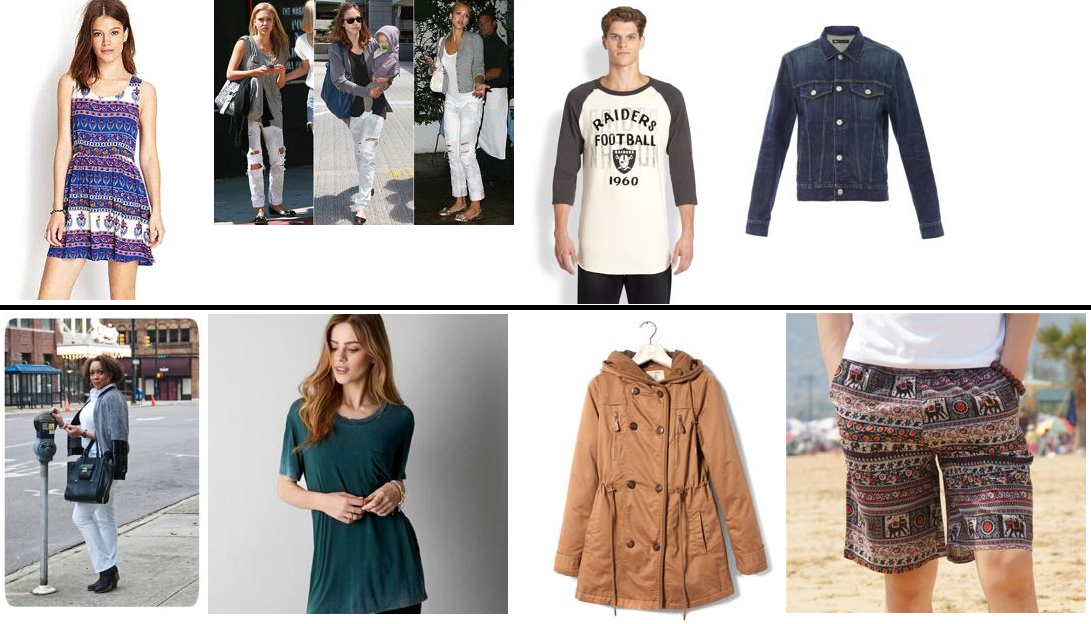
\includegraphics[width=\textwidth]{dataset.png}
\begin{itemize}
 \item 289222 images
 \item 48 classes (Hoodie, Jeans, Jumpsuit, \dots)
\end{itemize}
\end{frame}

\begin{frame}
\frametitle{Preprocessing}
\begin{itemize}
 \item Random crop to the smaller size (width or height)
 \item Resize to 227x227
\end{itemize}
\end{frame}

\section{Our solution}
\begin{frame}
\frametitle{Self-supervised Learning}
\begin{itemize}
 \item 70\% of the dataset
 \item Jigsaw Puzzle (3x3 tiles)
 \item AlexNet
 \item Optimizer: Adam with constant learning rate 0.0001
\end{itemize}
\end{frame}

\begin{frame}
\frametitle{Classification}
\begin{itemize}
 \item AlexNet initialized with the weights of the self-supervised part
 \item Optimizer: Adam with constant learning rate 0.001
\end{itemize}
\end{frame}

\section{Results}
\begin{frame}
\frametitle{Results}

\end{frame}

\section{Conclusions}
\begin{frame}
\frametitle{Conclusions}

\end{frame}



\begin{frame}[plain]
\begin{center}
\LARGE Questions?
\end{center}
\end{frame}

\begin{frame}
This has to be presented:
\begin{itemize}
 \item Task description
 \item Motivation
 \item Challenges
 \item Prior work
 \item Your solution
 \item Results and analysis
 \item Conclusions
\end{itemize}
\end{frame}

\end{document}